\documentclass{standalone}
% \documentclass[12pt,a3paper]{article}
\usepackage{tikz}
\usetikzlibrary{math}

\begin{document}
\pagestyle{empty}

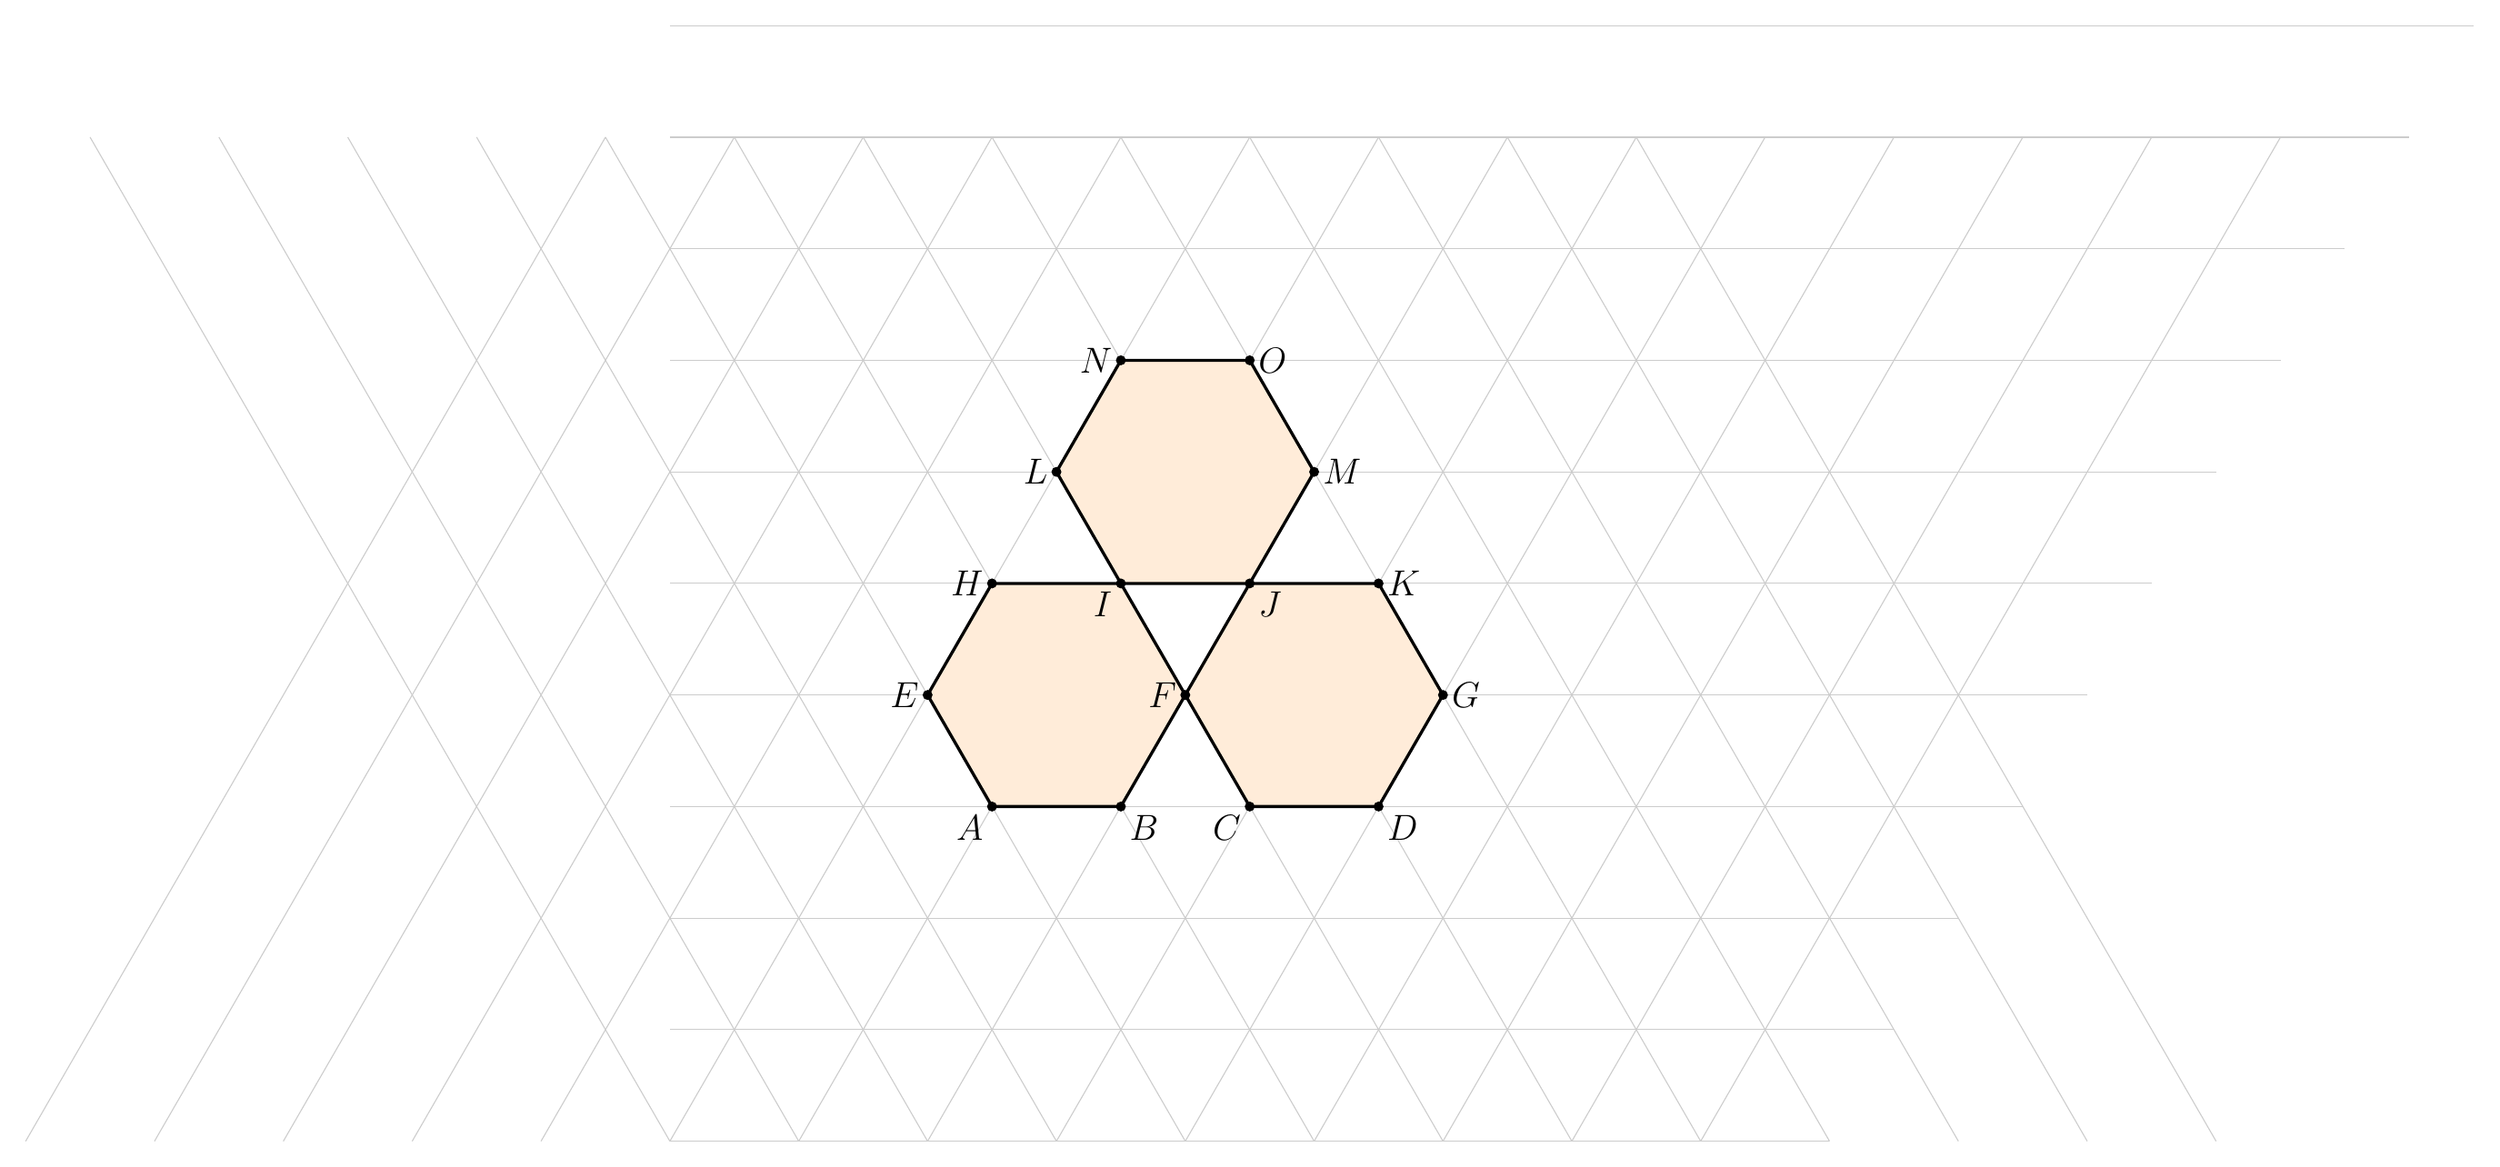
\begin{tikzpicture}[scale=1]

	\tikzmath{
		\r = 1.8;          % rayon (cm) — modifier pour agrandir/réduire
		\h = \r * 0.8660;  % r * sqrt(3)/2
		\hr = \r / 2;      % r/2
	}

	\begin{scope}[gray!40, thin]

		% Famille 1 : lignes horizontales (j fixé, i varie)
		% y = j*h,  x = i*r + j*r/2
		\foreach \j in {-2,-1,0,1,2,3,4,5,6,7,8}{
				\draw ({-\r }, {\j*\h}) -- ({9*\r + \j*\hr}, {\j*\h});
			}

		% Famille 2 : lignes direction (r, h) — obliques montant droite
		% i fixé : points (i*r + j*r/2, j*h)
		\foreach \i in {-5,-4,-3,-2,-1,0,1,2,3,4,5,6,7,8}{
				\draw ({\i*\r-2*\hr}, {0-2*\h}) -- ({\i*\r + 7*\hr}, {7*\h});
			}

		% Famille 3 : lignes direction (-r/2, h) — obliques montant gauche
		% k = i+j fixé : x = k*r - j*r/2,  y = j*h
		\foreach \k in {-2,-1,0,1,2,3,4,5,6,7,8,9,10}{
				\draw ({\k*\r+2*\hr}, {0-2*\h}) -- ({\k*\r - 7*\hr}, {7*\h});
			}

	\end{scope}


	\tikzset{hex/.style={
				fill=orange!15,
				draw=black,
				line width=1.2pt
			}}

	\draw[hex] ({2*\r - \hr}, \h)
	-- ({2*\r + \hr}, \h)
	-- ({3*\r},       {2*\h})
	-- ({2*\r + \hr}, {3*\h})
	-- ({2*\r - \hr}, {3*\h})
	-- ({1*\r},       {2*\h})
	-- cycle;

	\draw[hex] ({4*\r - \hr}, \h)
	-- ({4*\r + \hr}, \h)
	-- ({5*\r},       {2*\h})
	-- ({4*\r + \hr}, {3*\h})
	-- ({4*\r - \hr}, {3*\h})
	-- ({3*\r},       {2*\h})
	-- cycle;

	\draw[hex] ({3*\r - \hr}, {3*\h})
	-- ({3*\r + \hr}, {3*\h})
	-- ({4*\r},       {4*\h})
	-- ({3*\r + \hr}, {5*\h})
	-- ({3*\r - \hr}, {5*\h})
	-- ({2*\r},       {4*\h})
	-- cycle;


	\tikzset{lbl/.style={font=\small\itshape}}

	\node[lbl, below left]  at ({2*\r-\hr}, \h)     {\Large $A$};
	\node[lbl, below right] at ({2*\r+\hr}, \h)     {\Large $B$};
	\node[lbl, left]        at ({1*\r},     {2*\h}) {\Large $E$};
	\node[lbl, left]        at ({2*\r-\hr}, {3*\h}) {\Large $H$};
	\node[lbl, left]        at ({3*\r},     {2*\h}) {\Large $F$};
	\node[lbl, below left]  at ({2*\r+\hr}, {3*\h}) {\Large $I$};
	\node[lbl, below left]  at ({4*\r-\hr}, \h)     {\Large $C$};
	\node[lbl, below right] at ({4*\r+\hr}, \h)     {\Large $D$};
	\node[lbl, right]       at ({5*\r},     {2*\h}) {\Large $G$};
	\node[lbl, right]       at ({4*\r+\hr}, {3*\h}) {\Large $K$};
	\node[lbl, below right] at ({4*\r-\hr}, {3*\h}) {\Large $J$};
	\node[lbl, left]        at ({2*\r},     {4*\h}) {\Large $L$};
	\node[lbl, right]       at ({4*\r},     {4*\h}) {\Large $M$};
	\node[lbl, left]        at ({3*\r-\hr}, {5*\h}) {\Large $N$};
	\node[lbl, right]       at ({3*\r+\hr}, {5*\h}) {\Large $O$};

	\tikzset{pt/.style={circle, fill=black, inner sep=1.4pt}}
	\foreach \x/\y in {
	{2*\r-\hr}/{\h},
	{2*\r+\hr}/{\h},
	{1*\r}/{2*\h},
	{3*\r}/{2*\h},
	{5*\r}/{2*\h},
	{2*\r-\hr}/{3*\h},
	{2*\r+\hr}/{3*\h},
	{4*\r-\hr}/{\h},
	{4*\r+\hr}/{\h},
	{4*\r+\hr}/{3*\h},
	{4*\r-\hr}/{3*\h},
	{2*\r}/{4*\h},
	{4*\r}/{4*\h},
	{3*\r-\hr}/{5*\h},
	{3*\r+\hr}/{5*\h}
	}{
	\node[pt] at (\x, \y) {};
	}

\end{tikzpicture}

\end{document}

\documentclass{standalone}
\usepackage{tikz,ifthen}
\usepackage{tkz-tab}
\usepackage{xcolor}
\usepackage{amsmath}
\begin{document}

\begin{tikzpicture}
	\tkzTabInit[espcl=1.7]{$x$ / 1 , $f(x) = ax^2 + bx + c$ / 1}{$-\infty$, , $+\infty$}
	\tkzTabLine{,, -, }
\end{tikzpicture}

\end{document}
